\documentclass[tikz]{standalone}

\usepackage{amsfonts}
\usepackage{amsmath}
\usepackage{braket}

\usepackage{tikz}
\usetikzlibrary{calc, decorations, positioning}

\definecolor{googleR}{HTML}{DB4437}
\definecolor{googleG}{HTML}{0F9D58}
\definecolor{googleB}{HTML}{4285F4}

% main document
\begin{document}
	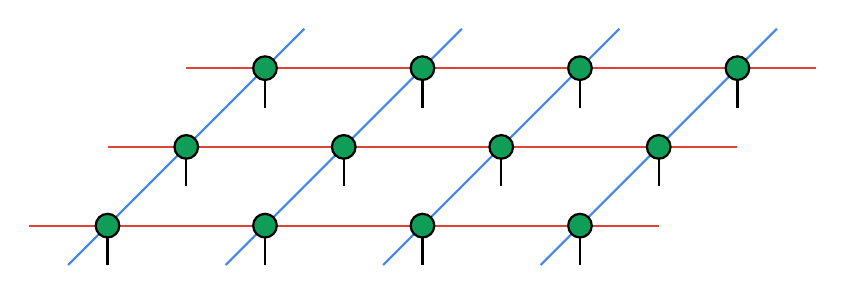
\begin{tikzpicture}[]
      \foreach \y in {-0.75, -0.25, +0.25} {
        \foreach \x in {-1.5, -0.5, +0.5, +1.5} {
          \begin{scope}[shift = {(2*\x + 2*\y, 2*\y)}]
            \draw[thick, googleR] (-1.00, 0) to (-0.00, 0);
            \draw[thick, googleR] (+0.00, 0) to (+1.00, 0);
            \draw[thick, googleB] (-0.50, -0.50) to (0, 0);
            \draw[thick, googleB] (0, 0) to (+0.50, +0.50);
            \draw[thick] (0, 0) to (0, -0.50);
            \draw[thick, fill = googleG] (0,0) circle (0.15);
            % \draw[thick, googleG] (-0.15, 0) to (+0.15, 0);
          \end{scope}
        }
      }
	\end{tikzpicture}
\end{document}

%%% Local Variables:
%%% mode: latex
%%% TeX-master: t
%%% End:
